\chapter{Recubridores}%
\label{cha:recubridores}
\section{El problema de elevación}%
\label{sec:el_problema_de_elevacion}
Fijada $p$, qué $f$'s tienen \underline{elevación} $\tilde{f}$. i.e: $p \circ \tilde{f} = f$ 
%TODO: Imagen
\begin{center}
    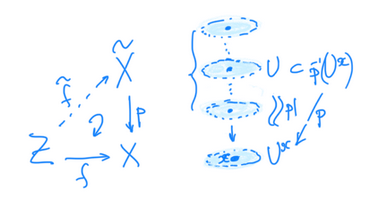
\includegraphics[scale=0.3]{images/problema_elevacion} 
\end{center}
\begin{defi}
$p$ es un \underline{recubridor} si $\forall x \in X,\ \underbrace{\exists U^x}_{\text{ab. \underline{trivializante}}} : p^{-1}\left( U^x \right) = \bigsqcup_{\lambda} U_{\lambda}$ y $\forall \lambda, p|: U_{\lambda} \rightarrow U^x$ homeomorfismo.
\end{defi}
Es un tipo especial de homeomorfismo local sobreyectivo y, por eso, identificación abierta.

\begin{ej}[¡Importantes!]
\begin{enumerate}
    \item La identificación \underline{antipodal}, $\pi: \mathbb{S} \rightarrow \mathbb{R}\mathrm{P}^n$,
    \[
    \forall x \in \mathbb{R}\mathrm{P}^n \underbrace{\exists U^x}_{\text{trivializante}} = \mathbb{R}\mathrm{P}^n \setminus \underbrace{H}_{\text{hiperplano}}\; \land \;\pi^{-1}\left( U^x \right) = \mathbb{S}^n\setminus \pi^{-1}H = S_+ \sqcup S_-  
    \]
    hemisferios abiertos.

    Ya se ilustró convenientemente en su lección. ¿Qué se tiene para $n = 1$?

    \item La identificación \underline{exponencial}, $p: \mathbb{R} \rightarrow \mathbb{S}^1: \theta \mapsto e^{2ni\theta} = \left( \cos 2\pi\theta, \sin 2\pi\theta \right)$.
    %TODO: Imagen
    \begin{center}
        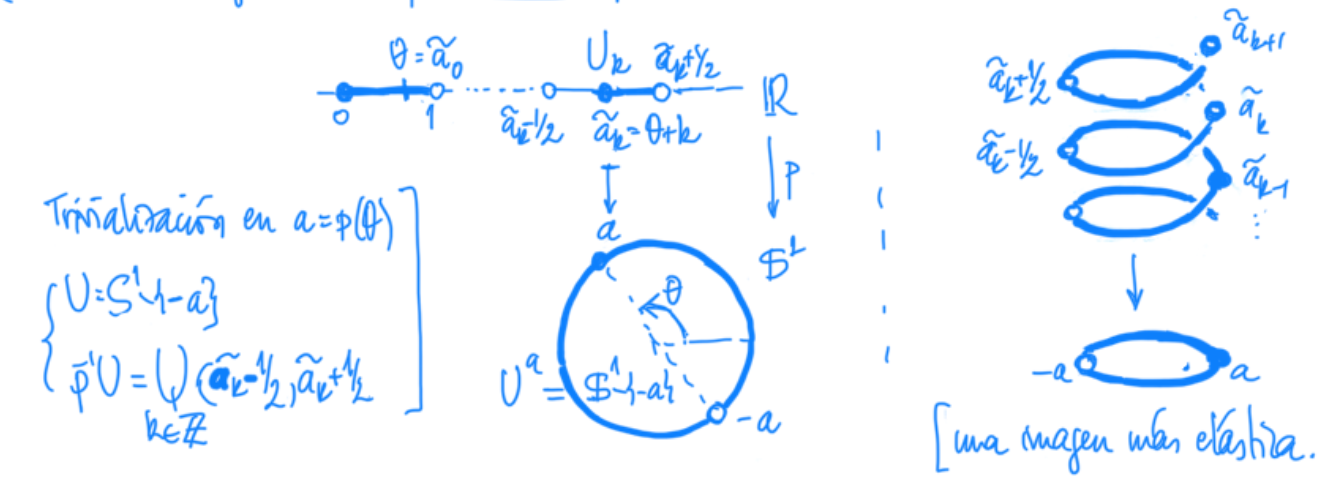
\includegraphics[scale=0.2]{images/identificacion_exponencial} 
    \end{center}
\end{enumerate} 
\end{ej}

\section{Unicidad de elevación}%
\label{sec:unicidad_de_elevacion}
\begin{prop}
Si $Z$ es conexo, dos elevaciones que coinciden en algún puntos son iguales.
\end{prop}
\begin{demo}
    $A = \{z \in Z: \tilde{f}_1 \left( z \right) = \tilde{f}_2\left( z \right)\}, p \circ \tilde{f}_1 = f$.
    \begin{align*}
        \underbrace{x}_{f\left( z \right)} \in U^x,\ p^{-1} U^x &= \bigsqcup_{\lambda} U_{\lambda} \text{ (trivialización)} \Rightarrow \tilde{f}_i\left( z \right) \in p ^{-1}U^x\; \land \;\exists!\lambda_i: \tilde{f}_i\left( z \right) \in U_{\lambda_i}\\
        &\Rightarrow \forall \eta \in W^z = \tilde{f}_1^{-1}\left( U_{\lambda_1} \right) \cap \tilde{f}_2^{-1} \left( U_{\lambda_2} \right): \hat{f}_1\left( \eta \right) = \hat{f}_2\left( \eta \right) \stackrel{(*)}{\Leftrightarrow} \lambda_1 = \lambda_2 (**)
    .\end{align*}
    $(*)$ debido a: 
    \begin{itemize}
        \item $\Rightarrow) U_{\lambda}$'s disjuntos. 
        \item $\Leftarrow) p \tilde{f}_1 = p \tilde{f}_2$ y $p|_{U_\lambda}$ 1-1.
    \end{itemize}

    Por tanto, 
    \begin{align*}
        \underbrace{\text{Ab.}}_{A} W^z \subset A \text{ si } z \in A: \tilde{f}_1\left( z \right) = \tilde{f}_2\left( z \right) &\stackrel{(**)}{\Rightarrow} \lambda_1 = \lambda_2 \Rightarrow \tilde{f}_1\left( W^z \right)\ \land \ \tilde{f}_2\left( W^z \right) \subset U_{\lambda_1} = U_{\lambda_2} \xrightarrow{p|} \underbrace{U^x }_{\text{iny.}}\\
        &\Rightarrow \forall \eta \in W^z: \tilde{f}_1\left( \eta \right),\ \tilde{f}_2\left( \eta \right) \mapsto \tau?\left( z \right) \Rightarrow \tilde{f}_1\left( \eta \right) = \tilde{f}_2\left( \eta \right)
    .\end{align*}
    y, 
    \begin{align*}
        \underbrace{\text{Cerr.}}_{A} W^z \subset Z \setminus A \text{ si } z \not\in A: \tilde{f}_1\left( z \right) \neq \tilde{f}_2\left( z \right) &\stackrel{(**)}{\Rightarrow} \lambda_1 \neq \lambda_2 \Rightarrow \tilde{f}_1\left( W^z \right) \cap \tilde{f}_2\left( W^z \right) \subset U_{\lambda_1} \cap U_{\lambda_2} = \emptyset\\
        &\Rightarrow \forall \eta \in W^z: \tilde{f}_1\left( \eta \right) \neq \tilde{f}_2\left( \eta \right) 
    .\end{align*}
    Por tanto, 
    \[
        \exists \tilde{f}_1\left( z \right) = \tilde{f}_2\left( z \right) \Rightarrow \emptyset \neq A \stackrel[\text{cerr.}]{\text{ab.}}{\subset} Z \text{ conx.} \Rightarrow A = Z\; \land \;\tilde{f}_1 = \tilde{f}_2
    \]
\end{demo}

\section{Lema de elevacción}%
\label{sec:lema_de_elevaccion}
\begin{prop}
Tenemos que:
\[
\begin{cases}
    f = H: Y \times \left[ 0, 1 \right] \rightarrow X \text{ (homotopía)} \\
    \exists \tilde{H}_0 \text{ elevación de } H_0: Y \rightarrow X
\end{cases} \Rightarrow \exists \tilde{H} \text{ elevación, } \left( \tilde{H} \right)_0 = \tilde{H}_0
\]
\end{prop}
\begin{demo}
\begin{enumerate}
    \item \underline{Elevación semilocal}: $\forall y \in Y,\ \tilde{H}^y: V^y \times \left[ 0, 1 \right] \rightarrow \tilde{X}$ elevación de $H|_{V^y \times \left[ 0, 1 \right]}$.
    \begin{enumerate}
        \item $\{y\} \times \left[ 0, 1 \right] \subset \bigcup_{x} H^{-1}\left( U^x \right),\ p ^{-1} U^x = \bigsqcup_{\lambda} U_{\lambda}$ (trivialización en $x$) $\Rightarrow$
        \begin{align*}
            &\xRightarrow{\text{comp.}} \exists 0 = t_0 < t_1 < \ldots < t_r = 1: \{y\} \times \left[ t_{i - 1}, t_i \right] \subset H^{-1}\left( U^{x_i} \right)\\
            &\xRightarrow{\text{comp.}} \forall i,\ \exists V_i^y \times \left[ t_{i-1}, t_i \right] \subset H^{-1}\left( U^{x_i} \right)\\
            &\Rightarrow \exists V^y = V_1^y \cap \ldots \cap V_r^y: V^y \times \left[ t_{i - 1}, t_i \right] \stackrel{(*)}{\subset} H^{-1}\left( U^{x_i} \right)
        .\end{align*}

        \item Inducción, $i > 0: \exists \tilde{H}_0: V^y \times \{t_0\} \rightarrow \tilde{X}$ por hipótesis. 
        \begin{align*}
            \underline{i - 1 \rightarrow i}:\ &\exists H_{i - 1}^y \text{ en } V^y \times \left[ t_0, t_{i - 1?} \right] \Rightarrow \text{se puede extender a } V^y \times \left[ t_{i - 1}, t_i \right] \\
            (*) &\Rightarrow \begin{cases}
                H\left( y, t_{i - 1} \right) \in U^{x_i} \xRightarrow{\exists \lambda} \tilde{H}_{i - 1}^y \left( y, t_{i - 1} \right) \in U_{\lambda} \xRightarrow{\text{red. } V^y}\\
                \qquad \hat{H}_{i - 1}^y \left( V^y \times \left( t_{i - 1} \right) \right) \subset U_{\lambda} \rightarrow U^{x_i}\\
                \exists \left( p|_{U_{\lambda}}^{-1}\right) \circ H: V^y \times \left[ t_{i - 1}, t_i \right] \rightarrow U_{\lambda} \text{ elevación (de } H)
            \end{cases}\\
                &\Rightarrow p\circ\tilde{H}_{i - 1}^y = p \circ \left[ \left( p|_{U_{\lambda}}^{-1} \circ H \right) \right]: V^y \times \{t_{i - 1}\} \rightarrow U^{x_i}\\
                &\quad \xRightarrow{p|_{U_\lambda} \text{ iny.}} \tilde{H}_{i - 1}^y = \left( p|_{U_{\lambda}} \right)^{-1} \circ H \text{ en } V^y \times \{t_{i - 1}\}\\
                &\Rightarrow \left( p|_{U_{\lambda}}^{-1} \right) \circ H \text{ extiende } \tilde{H}_{i - 1}^y \text{ a } V^y \times \left[ t_{i - 1}, t_i \right] 
        .\end{align*}
    \end{enumerate}

    \item \underline{Elevación global}. Las locales $\{\tilde{H}^y: V^y \times \left[ 0, 1 \right] \rightarrow \tilde{X}\}_{y \in Y}$ encolan bien, pues coinciden en las intersecciones: $\forall y \in V^{y_1} \cap V^{y_2}$:
\end{enumerate}
\end{demo}

\begin{obs}
\begin{enumerate}
    \item La elevación de una aplicación $Y \rightarrow X$ sólo depende de su clase de homotopía.
    \item Todo camino $\sigma: \left[ 0, 1 \right] \rightarrow X$ tiene uan única elevación $\tilde{\sigma}$ con origen $\tilde{\sigma}\left( 0 \right) \in p^{-1}\left( \sigma\left( 0 \right) \right)$.
    \[
    \begin{rcases}
    \begin{rcases}
        \tilde{H}^{y_1} \left( y, \bullet \right)\\
        \tilde{H}^{y_2} \left( y, \bullet \right) 
    \end{rcases} \text{elevan } H\left( y, \bullet \right) : \{y\} \times \left[ 0, 1 \right] \\  
    \tilde{H}^{y_1} \left( y, 0 \right) = \tilde{H}_0\left( y \right) = \tilde{H}^{y_2} \left( y, 0 \right) \text{ 1\textsuperscript{er} paso ind.} 
    \end{rcases} \xRightarrow{\text{Uni. elevaccón.}} 
    \tilde{H}^{y_1} \left( y, t \right) = \tilde{H}^{y_2} \left( y, t \right),\ \forall z
    \]
\end{enumerate}
\end{obs}


\chapter{Cálculos mediante recubridores}%
\label{cha:calculos_mediante_recubridores}
Hemos visto ya que:
\begin{itemize}
    \item $\pi$(estrellado) $= \{1\},\ \pi\left( \mathbb{S}^n \right) = \{1\},\ n \ge 2 \Rightarrow \pi\left( \mathbb{R}^{n + 1} \setminus \{0\} \right) = \{1\}$.
    \item $\pi\left( \mathbb{P}^{n} \right) = \mathbb{Z}_2,\ n \ge  2$ (no demostrado)
    \item $\pi\left( \mathbb{S}^1 \right) = \mathbb{Z}$ (no demostrado).
    \begin{itemize}
        \item $\pi$(toro) $= \mathbb{Z} \times \mathbb{Z},\ \pi$(cilindro) $= \mathbb{Z}$.
        \item $\pi$(banda de Möbius) $= \mathbb{Z},\ \pi\left( \mathbb{R}^2 \setminus \{a\} \right) = \mathbb{Z}$.
    \end{itemize}
    Ahora toca demostrar $\pi\left( \mathbb{P}^{n} \right)$ y $\pi\left( \mathbb{S}^1 \right)$.
\end{itemize}

\section{Espacios proyectivos reales}%
\label{sec:espacios_proyectivos_reales_rec}
\begin{theo}
$\pi\left( \mathbb{P}^{n} \right) = \mathbb{Z}_2,\ n \ge 2$
\end{theo}
\begin{demo}
Usamos el recubridor antipodal $p : \mathbb{S}^n \rightarrow \mathbb{P}^{n}: \tilde{x}, -\tilde{x} \mapsto x = \left[ \tilde{x} \right] = \left[ - \tilde{x} \right]$. Punto base en $\mathbb{P}^{n}: x_0 = \left( 0 : \ldots : 1 \right);\ \sigma: \left[ 0, 1 \right] \rightarrow \mathbb{P}^{n},\ \sigma\left( 0 \right) = \sigma\left( 1 \right) = x_0,\ \tilde{x}_0 = \left( 0, \ldots, 1 \right)$. Ahora, por el lema de elevación:
\[
    \Rightarrow \exists! \tilde{\sigma}: \left[ 0, 1 \right] \rightarrow \mathbb{S}^{n},\ p\tilde{\sigma} = \sigma,\ \tilde{\sigma} = \tilde{x}_0\; \land \;\tilde{\sigma}\left( 1 \right) \in p^{-1}\left( x_0 \right) = \{\tilde{x}_0, -\tilde{x}_0\}  
\]
No veces? lazo.
\begin{enumerate}
    \item $\tilde{\sigma}\left( 1 \right) = \tilde{x}_0 \xRightarrow{\mathbb{S}^{n} \text{ simple conx.}} \exists \tilde{H}_s: \tilde{\sigma} \stackrel{x_0}{\simeq} \tilde{x}_0 \Rightarrow \exists p \circ \tilde{H}_s: \sigma \stackrel{x_0}{\simeq} x_0 \Rightarrow \left[ \sigma \right] = 1 \in \pi\left( \mathbb{P}^{n}, x_0 \right)$. 

    \item $\tilde{\sigma} \left( 1 \right) = -\tilde{x}_0 \xRightarrow{\mathbb{S}^{n} \text{ simple conx.}} \exists \tilde{H}_s: \tilde{\sigma} \stackrel{\tilde{x}_0,-\tilde{x}_0}{\simeq} \tilde{\alpha} = \left( 0, \ldots, 0, \sin \pi t, \cos \pi t \right) \Rightarrow \exists p \circ H_s: \sigma \stackrel{x_0}{\simeq} \alpha = p \circ \tilde{\alpha}$, lazo de base $x_0,\ \alpha\left( 0 \right) = \alpha\left( 1 \right) = x_0$. 

    \item Tenemos:
    %TODO: Imagen
    \begin{center}
        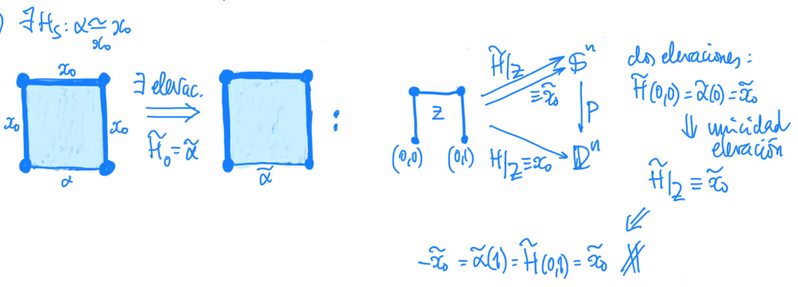
\includegraphics[scale=0.3]{images/rec_esp_proy_r} 
    \end{center}

    \item[1. 2. 3.] $\Rightarrow \pi\left( \mathbb{P}^{n}, x_0 \right)$ tiene dos elementos distintos dependiendo del extremo de la elevación $\Rightarrow$ 
        \[
        \boxed{\pi\left( \mathbb{P}^{n}, x_0 \right) = \mathbb{Z}_2}.
        \]
\end{enumerate}
\end{demo}

\section{La circunferencia}%
\label{sec:la_circunferencia}
\begin{theo}
$\pi\left( \mathbb{S}^{1} \right) = \mathbb{Z}$.
\end{theo}
\begin{obs}
$\mathbb{S}^{1} = \mathbb{P}^{1}$.
\end{obs}
\begin{demo}
    Usamos el recubridor exponencial $p: \mathbb{R} \rightarrow \mathbb{S}^{1}: \theta \mapsto \left( \cos 2 \pi \theta, \sin 2 \pi \theta \right)$. Punto base $x_0 \in \mathbb{S}^{1},\ \forall \sigma: \left[ 0, 1 \right] \rightarrow \mathbb{S}^{1},\ s\left( 0 \right) = \sigma\left( 1 \right) = x_0$. Por el lema de elevación:
    \[
    \Rightarrow \exists \tilde{\sigma} : \left[ 0, 1 \right] \rightarrow \mathbb{R}^{}, p \tilde{\sigma} = \sigma \Rightarrow p \tilde{\sigma} \left( 1 \right) = \sigma\left( 1 \right) = \sigma\left( 0 \right) = p \tilde{\sigma} \left( 0 \right) \Rightarrow \tilde{\sigma} \left( 1 \right) = \tilde{\sigma} \left( 0 \right) + k,\ k \in \mathbb{Z}
    \]

\begin{theo}
    El \underline{nº de vueltas}:
    \begin{align*}
        \#: \pi\left( \mathbb{S}^{1}, x_0 \right) &\rightarrow \mathbb{Z}\\
        \left[ \sigma \right] &\mapsto \# \sigma = \tilde{\sigma}\left( 1 \right) - \tilde{\sigma}\left( 0 \right) 
    .\end{align*}
    es isomorfismo de grupos bien definido.
\end{theo}
\begin{demo}
    \begin{enumerate}
        \item $k = \tilde{\sigma} \left( 1 \right) - \tilde{\sigma} \left( 0 \right)$ no depende de $\tilde{\sigma}$. 
        \begin{align*}
            p \tilde{\tau} = \sigma = p \tilde{\sigma} &\Rightarrow \tilde{\tau} \left( 0 \right) = \tilde{\sigma} \left( 0 \right) + l \Rightarrow \begin{cases}
                \tilde{\tau}\\
                \tilde{\sigma} + l
            \end{cases} \parbox{5em}{elevan $\sigma$\\ coinciden\\ en $t = 0$} \xRightarrow{\text{uni. elev.}} \tilde{\tau} = \tilde{\sigma} + l\\
            &\Rightarrow k = \tilde{\sigma}\left( 1 \right) - \tilde{\sigma} \left( 0 \right) = \left( \tilde{\tau} \left( 1 \right) - l \right) - \left( \tilde{\tau} \left( 0 \right) - l \right) = \tilde{\tau} \left( 1 \right) - \tilde{\tau} \left( 0 \right) 
        .\end{align*}

        \item $k$ no depende de homotopía de lazos, luego $\#$ está bien definido. Sea $H_s: \sigma \simeq \tau$ y $H_s\left( 1 \right) = H_s\left( 0 \right),\ \forall s$:
        \begin{align*}
            &\Rightarrow \exists \tilde{H}_s: \tilde{\sigma} \simeq \tilde{\tau} \text{ entre elevaciones de } \sigma\; \land \;\tau\\
            &\Rightarrow s \mapsto \underbrace{\tilde{H}_s\left( 1 \right)}_{\xrightarrow{p} H_s\left( 1 \right) }  \setminus \underbrace{\tilde{H}_s\left( 0 \right)}_{\xrightarrow{p} H_s\left( 0 \right)} \in \mathbb{Z} \xRightarrow{\text{cont.}} \tilde{H}_s\left( 1 \right) - \tilde{H}_s\left( 0 \right) \equiv cte.\\
            &\Rightarrow k = \tilde{\sigma} \left( 1 \right) - \tilde{\sigma} \left( 0 \right) = \tilde{H}_0\left( 1 \right) - \tilde{H}_0\left( 0 \right) \stackrel{cte.}{=} \tilde{H}_1\left( 1 \right) - \tilde{H}_1\left( 0 \right) = \tilde{\tau} \left( 1 \right) - \tilde{\tau} \left( 0 \right)  
        .\end{align*}

        \item $\#$ es isomorfismo. Sea $\# \sigma = \tilde{\sigma} \left( 1 \right) - \tilde{\sigma} \left( 0 \right)$ y $\# \tau = \tilde{\tau} \left( 1 \right) - \tilde{\tau} \left( 0 \right)$ y:
        \begin{align*}
            \tau\left( 0 \right) = \tau\left( 1 \right) = p \tilde{\sigma} \left( 1 \right) &\Rightarrow \tilde{\sigma} \left( 1 \right) \text{ cond. inicial elev.} \\
            &\Rightarrow \exists \tilde{\tau} : \underline{\tilde{\tau} \left( 0 \right) = \tilde{\sigma} \left( 1 \right)} \Rightarrow \tilde{\sigma} * \tilde{\tau} = \tilde{\sigma * \tau} 
        .\end{align*}
        Entonces:
        \begin{align*}
            \# \left( \sigma * \tau \right) &= \tilde{\sigma * \tau} \left( 1 \right) - \tilde{\sigma * \tau} \left( 0 \right) = \tilde{\sigma} * \tilde{\tau} \left( 1 \right) - \tilde{\sigma} * \tilde{\tau} \left( 0 \right) = \tilde{\tau} \left( 1 \right) - \tilde{\sigma} \left( 0 \right) =\\
            &= \left( \tilde{\tau} \left( 1 \right) - \tilde{\tau} \left( 0 \right) \right) + \left( \tilde{\sigma} \left( 1 \right) - \tilde{\sigma} \left( 0 \right) \right) = \# \tau + \# \sigma
        .\end{align*}

        \item $\#$ es suprayectiva: 
        \[
        \# \left( \cos 2 \pi k t, \sin 2 \pi k t \right) = k t|_0^1 = k 
        \]
        (Recorrer $\mathbb{S}^{1}\ k$ veces)

        \item $\#$ es 1-1:
        \[
        0 = \# \sigma = \tilde{\sigma} \left( 1 \right) - \tilde{\sigma} \left( 0 \right) \Rightarrow \begin{cases}
            \tilde{\sigma\left( 1 \right)} = \tilde{\sigma} \left( 0 \right) \Rightarrow \begin{rcases}
                H_s\left( 0 \right) = p \tilde{\sigma} \left( 0 \right) = \sigma\left( 0 \right) = \sigma\left( 0 \right) = x_0\\
                H_s\left( 1 \right) = p \tilde{\sigma} \left( 1 \right) = \sigma\left( 1 \right) = x_0
            \end{rcases}(*)\\\\

            \underbrace{p\left( \left( 1 - s \right) \tilde{\sigma} \left( t \right) + s \tilde{\sigma} \left( 0 \right) \right)}_{H_s\left( t \right)} : \sigma \stackrel[(*)]{x_0}{\simeq} x_0 
        \end{cases} 
        \]
        [$\Rightarrow \left( \sigma \right) = 1 \in \pi \left( \mathbb{S}^{1}, x_0 \right)$]
    \end{enumerate}
\end{demo}
\end{demo}

